% Original schematic figures for the flashcards.
% Compile with LuaLaTeX; each tikzpicture is one page.
% Geometry: Schuett--Shioda, Elliptic Surfaces, sections 4 and 6.
% Drawing: PGF/TikZ manual, paths, plots, nodes, and foreach.
\documentclass[tikz,border=8pt]{standalone}
\usepackage{amsmath}
\definecolor{curveblue}{HTML}{156082}
\definecolor{curveorange}{HTML}{A84216}
\definecolor{curvegreen}{HTML}{287443}
\tikzset{
  curve/.style={line width=1.4pt,curveblue},
  component/.style={circle,draw=curveblue,line width=1pt,fill=white,
    minimum size=8mm,inner sep=0pt,font=\large},
  identity/.style={component,double,double distance=1.4pt},
  edge/.style={line width=1.1pt,curveblue},
  every picture/.style={font=\large}
}
\begin{document}
\pagecolor{white}
% 01: smooth genus-one curve, topological schematic.
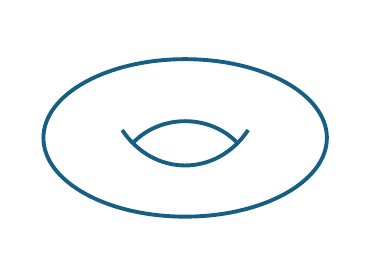
\begin{tikzpicture}
  \path[use as bounding box] (-2,-1.4) rectangle (2,1.4);
  \draw[curve] (0,0) ellipse (1.8 and 1.0);
  \draw[curve] (-.8,.1) .. controls (-.4,-.5) and (.4,-.5) .. (.8,.1);
  \draw[curve] (-.65,-.05) .. controls (-.3,.3) and (.3,.3) .. (.65,-.05);
\end{tikzpicture}
% 02: irreducible nodal curve.
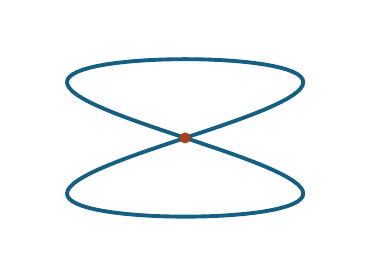
\begin{tikzpicture}
  \path[use as bounding box] (-2,-1.4) rectangle (2,1.4);
  \draw[curve] plot[domain=0:360,samples=121] ({1.5*sin(2*\x)},{sin(\x)});
  \fill[curveorange] (0,0) circle (2pt);
\end{tikzpicture}
% 03: irreducible cuspidal curve.
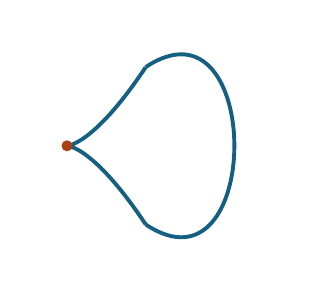
\begin{tikzpicture}
  \path[use as bounding box] (-.5,-1.5) rectangle (3,1.5);
  \draw[curve] plot[domain=-1:1,samples=101] ({\x*\x},{\x*\x*\x});
  \draw[curve] (1,1) .. controls (2.5,2) and (2.5,-2) .. (1,-1);
  \fill[curveorange] (0,0) circle (2pt);
\end{tikzpicture}
% 04: two components, two transverse intersection points.
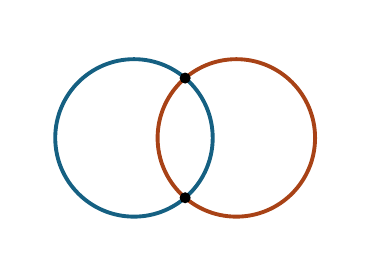
\begin{tikzpicture}
  \path[use as bounding box] (-2,-1.4) rectangle (2,1.4);
  \draw[curve] (-.65,0) circle (1);
  \draw[curve,curveorange] (.65,0) circle (1);
  \fill (0,.75993) circle (2pt);
  \fill (0,-.75993) circle (2pt);
\end{tikzpicture}
% 05: two tangent components.
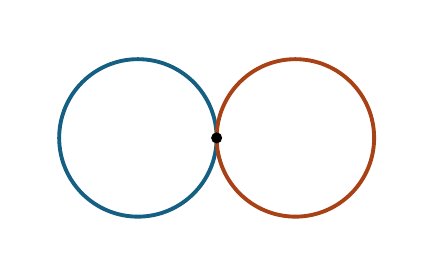
\begin{tikzpicture}
  \path[use as bounding box] (-2.4,-1.4) rectangle (2.4,1.4);
  \draw[curve] (-1,0) circle (1);
  \draw[curve,curveorange] (1,0) circle (1);
  \fill (0,0) circle (2pt);
\end{tikzpicture}
% 06: three components, three distinct intersections. Strokes are curves.
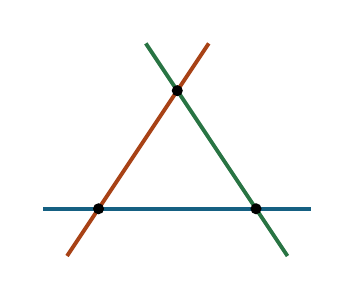
\begin{tikzpicture}
  \path[use as bounding box] (-1.9,-.8) rectangle (1.9,2.3);
  \draw[curve] (-1.7,0)--(1.7,0);
  \draw[curve,curveorange] (-1.4,-.6)--(.4,2.1);
  \draw[curve,curvegreen] (1.4,-.6)--(-.4,2.1);
  \foreach \p in {(-1,0),(1,0),(0,1.5)} \fill \p circle (2pt);
\end{tikzpicture}
% 07: three components through one point.
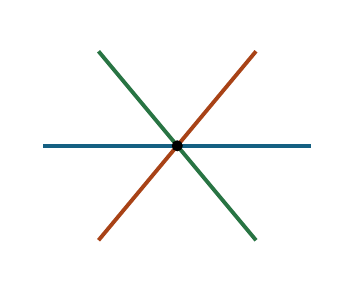
\begin{tikzpicture}
  \path[use as bounding box] (-1.9,-1.5) rectangle (1.9,1.5);
  \draw[curve] (-1.7,0)--(1.7,0);
  \draw[curve,curveorange] (-1,-1.2)--(1,1.2);
  \draw[curve,curvegreen] (-1,1.2)--(1,-1.2);
  \fill (0,0) circle (2pt);
\end{tikzpicture}
% 08: a cycle; vertices are components, labels are multiplicities.
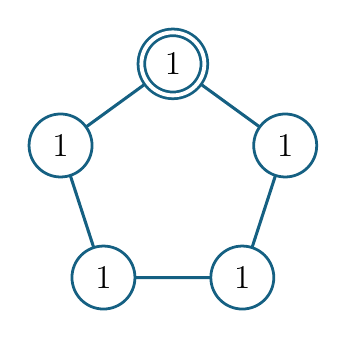
\begin{tikzpicture}
  \foreach \i in {0,...,4} \coordinate (p\i) at ({90+72*\i}:1.5);
  \draw[edge] (p0)--(p1)--(p2)--(p3)--(p4)--cycle;
  \node[identity] at (p0) {1};
  \foreach \i in {1,...,4} \node[component] at (p\i) {1};
\end{tikzpicture}
% 09: affine D4.
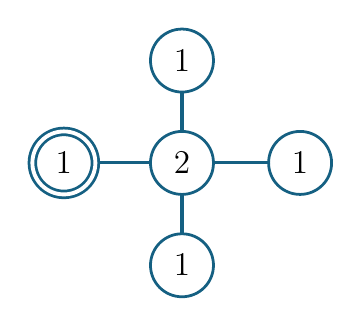
\begin{tikzpicture}
  \draw[edge] (-1.5,0)--(1.5,0) (0,-1.3)--(0,1.3);
  \node[component] at (0,0) {2};
  \node[identity] at (-1.5,0) {1};
  \node[component] at (1.5,0) {1};
  \node[component] at (0,1.3) {1};
  \node[component] at (0,-1.3) {1};
\end{tikzpicture}
% 10: affine D7; four double components, hence I3-star.
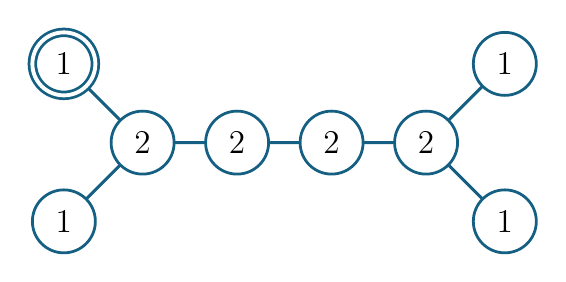
\begin{tikzpicture}
  \draw[edge] (0,0)--(3.6,0)
    (-1,1)--(0,0)--(-1,-1) (4.6,1)--(3.6,0)--(4.6,-1);
  \foreach \x in {0,1.2,2.4,3.6} \node[component] at (\x,0) {2};
  \node[identity] at (-1,1) {1};
  \node[component] at (-1,-1) {1};
  \node[component] at (4.6,1) {1};
  \node[component] at (4.6,-1) {1};
\end{tikzpicture}
% 11: affine E6, three arms of length two.
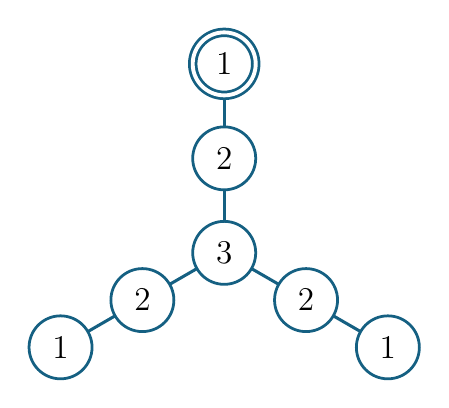
\begin{tikzpicture}
  \foreach \a in {90,210,330} {
    \draw[edge] (0,0)--(\a:2.4);
    \node[component] at (\a:1.2) {2};
  }
  \node[component] at (0,0) {3};
  \node[identity] at (90:2.4) {1};
  \node[component] at (210:2.4) {1};
  \node[component] at (330:2.4) {1};
\end{tikzpicture}
% 12: affine E7, arm lengths 3,3,1.
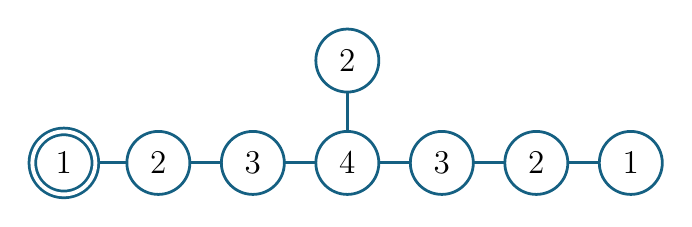
\begin{tikzpicture}
  \draw[edge] (-3.6,0)--(3.6,0) (0,0)--(0,1.3);
  \node[component] at (0,0) {4};
  \node[component] at (0,1.3) {2};
  \foreach \x/\m in {-2.4/2,-1.2/3,1.2/3,2.4/2,3.6/1}
    \node[component] at (\x,0) {\m};
  \node[identity] at (-3.6,0) {1};
\end{tikzpicture}
% 13: affine E8, arm lengths 5,2,1.
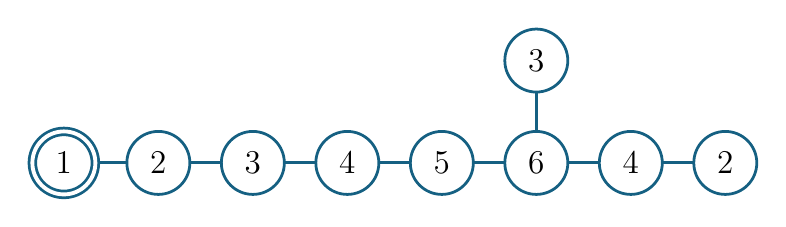
\begin{tikzpicture}
  \draw[edge] (-6,0)--(2.4,0) (0,0)--(0,1.3);
  \node[component] at (0,0) {6};
  \node[component] at (0,1.3) {3};
  \foreach \x/\m in {-4.8/2,-3.6/3,-2.4/4,-1.2/5,1.2/4,2.4/2}
    \node[component] at (\x,0) {\m};
  \node[identity] at (-6,0) {1};
\end{tikzpicture}
\end{document}
